\section{Proposed ClimateGuardian AI Framework}
\label{sec:framework}
\subsection{System Overview}
The ClimateGuardian AI framework is structurally bifurcated to address both rigorous scientific evaluation and operational deployment feasibility. 

\begin{figure*}[!t]
\centering
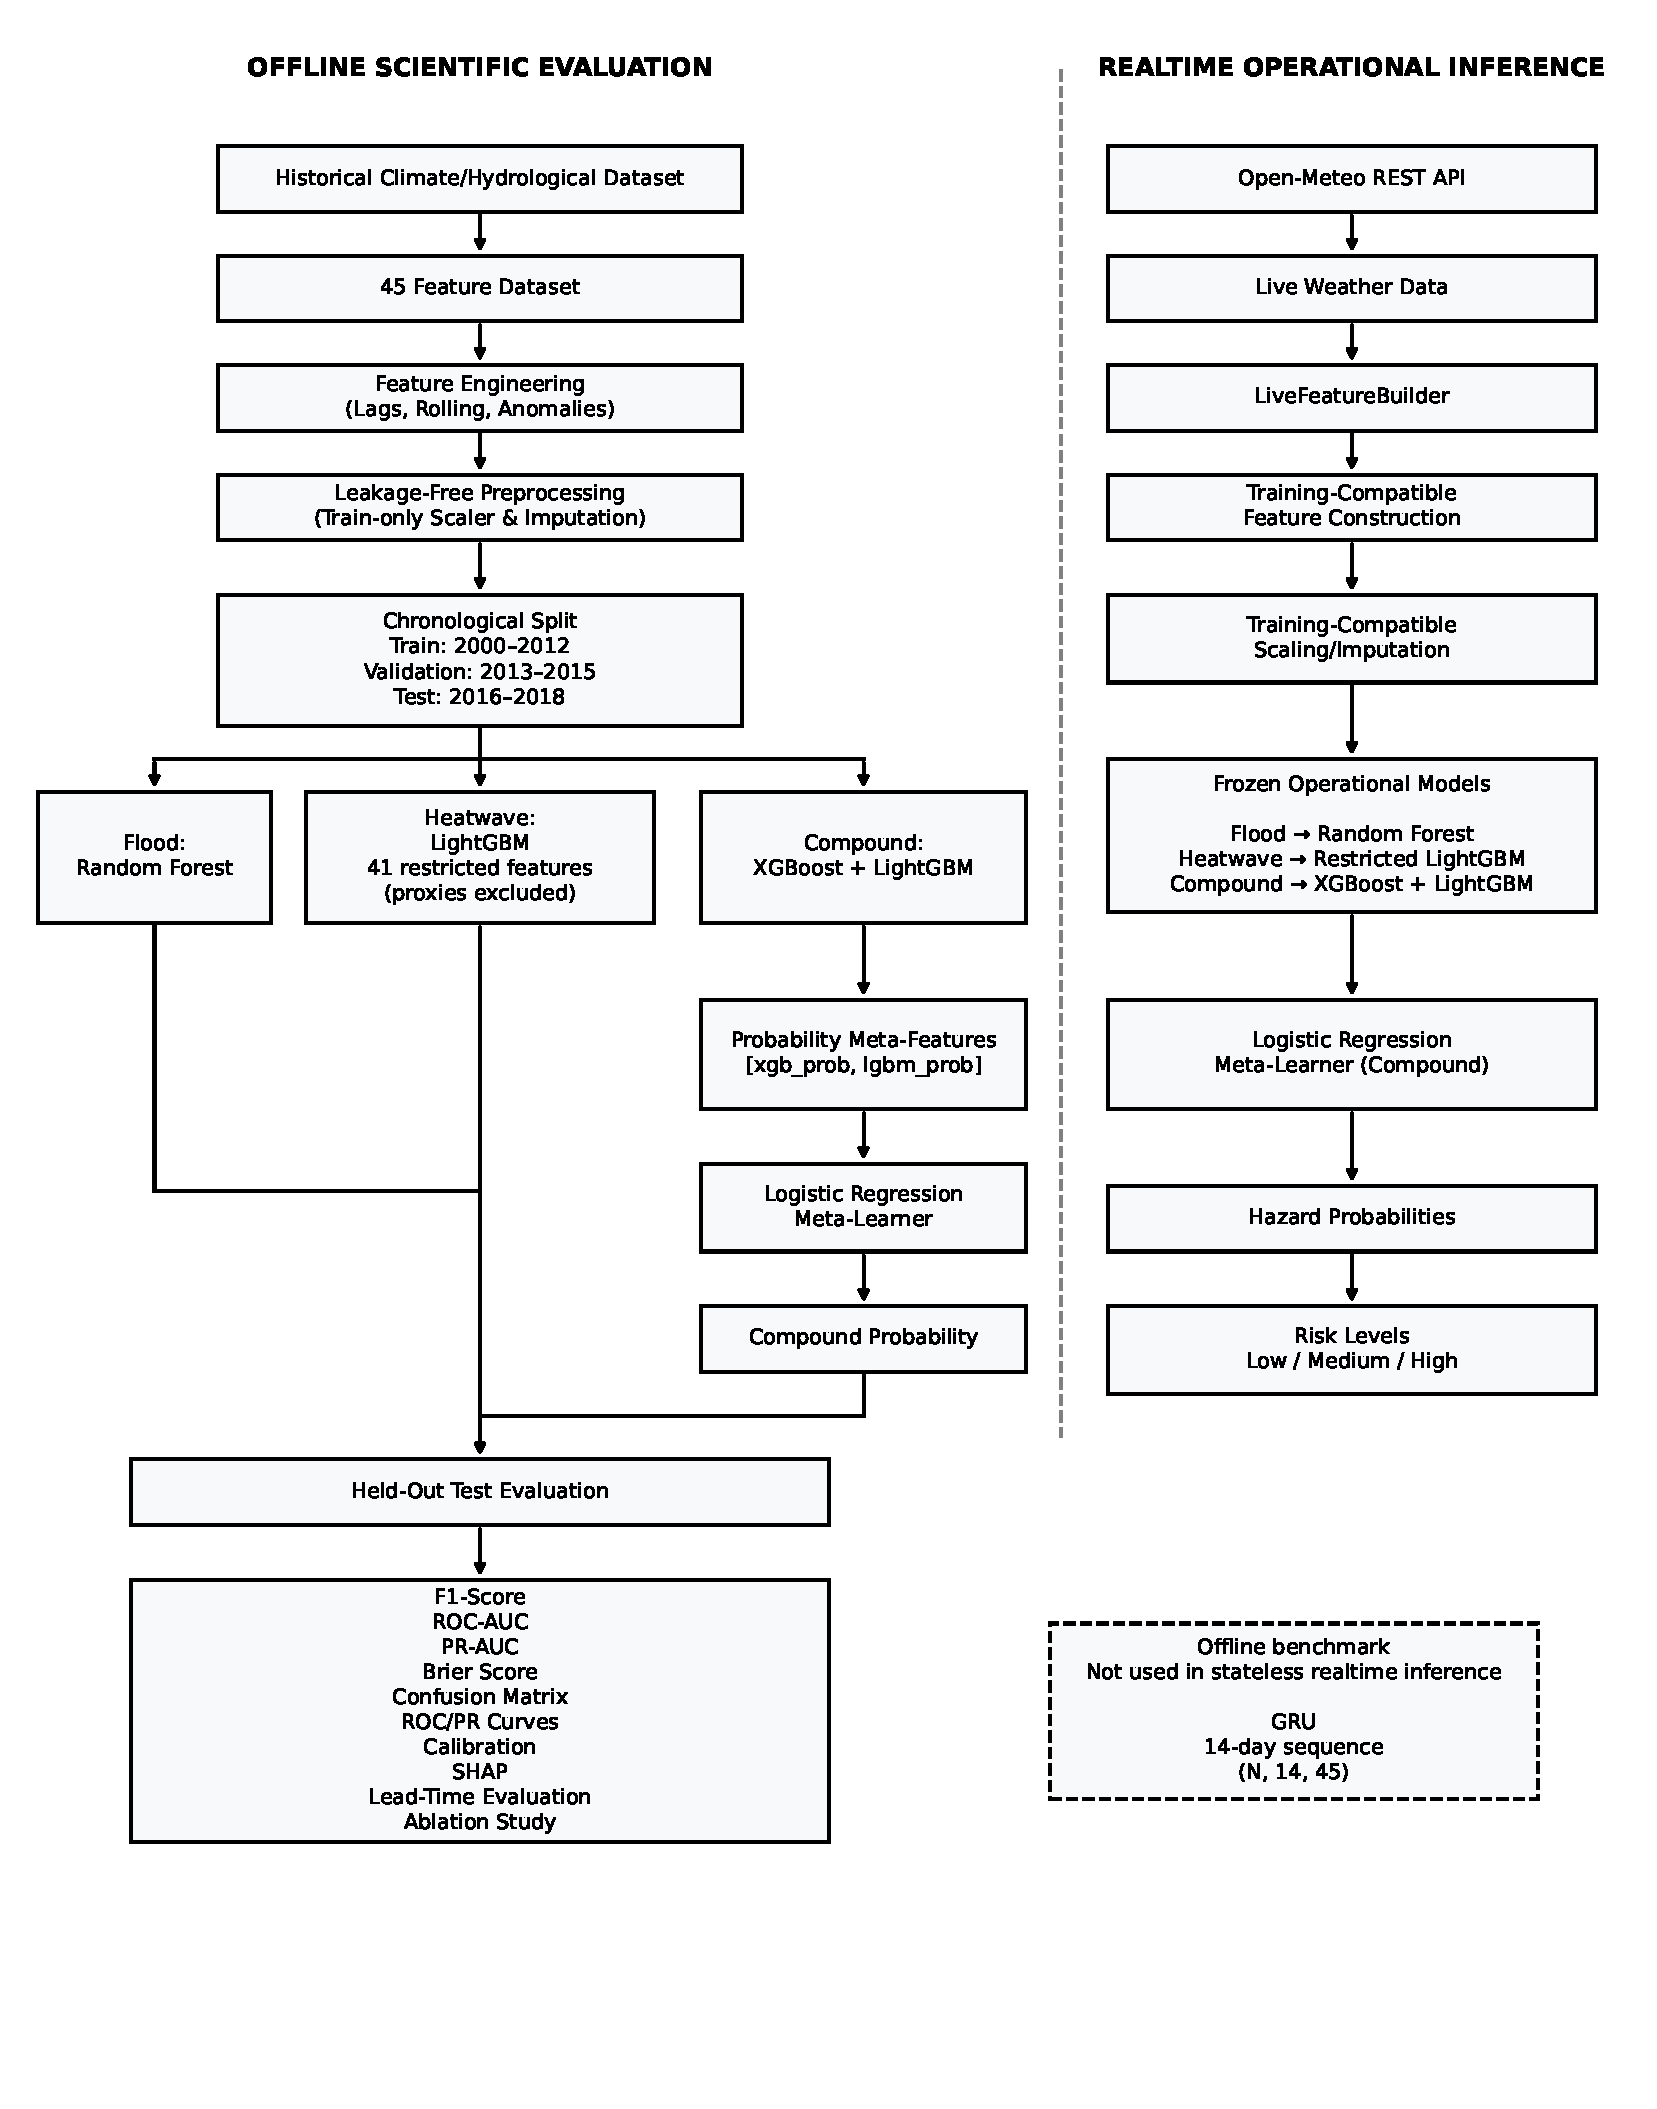
\includegraphics[width=\textwidth,height=0.85\textheight,keepaspectratio]{../Paper_Figures/Fig_01_Architecture.pdf}
\caption{Architecture of the ClimateGuardian AI framework showing the offline scientific evaluation pipeline and stateless realtime inference path.}
\label{fig:system_architecture}
\end{figure*}

As illustrated in Fig.~\ref{fig:system_architecture}, the offline environment processes historical data arrays, engineering required feature spaces and enforcing chronological splitting protocols for model training and benchmark evaluations. Conversely, the operational environment is entirely stateless, extracting instantaneous weather observations via API interfaces, structuring them dynamically, and generating predictive risk probabilities without accessing a persistent local database. 

\subsection{Data Sources}
The core historical hydro-climatic dataset integrates meteorological and hydrological phenomena into a unified daily representation (Table~\ref{tab:dataset}). 

\begin{table}[htbp]
\caption{Dataset Statistics (2000--2018)}
\begin{center}
\begin{tabular}{ll}
\toprule
\textbf{Metric} & \textbf{Value} \\
\midrule
Total Observations & 6,940 \\
Features & 45 \\
Flood Positives & 1,880 (27.09\%) \\
Heatwave Positives & 510 (7.35\%) \\
Compound Positives & 255 (3.67\%) \\
Missing Feature Values & 30 \\
\bottomrule
\end{tabular}
\label{tab:dataset}
\end{center}
\end{table}

Spanning from January 1, 2000, through December 31, 2018, the dataset contains 6,940 daily records defined across 45 continuous features. Climate variables include precipitation, temperature profiling, surface pressure, wind vectors, and evaporation. Hydrological inputs encompass surface runoff, total runoff, and soil moisture gradients.

\subsection{Feature Engineering}
To provide the stateless machine learning models with necessary temporal context, the base continuous features were systematically expanded. Standardized historical anomaly features were constructed to map deviations from established training norms. Furthermore, temporal aggregations---including 3-day, 5-day, 7-day, and 14-day rolling window statistics---were engineered to quantify accumulated environmental pressures prior to the instantaneous observation. Sequential lagged features ($t-1$, $t-2$, $t-3$) were directly appended to capture immediate short-term derivatives. 

\subsection{Multi-Hazard Target Formulation}
Three explicit predictive targets were algorithmically derived to form the hazard evaluation suite. Flood Risk operates as a binary target mapped from historical inundation and precipitation thresholds. Heatwave Risk identifies periods of severe temperature persistence. Compound Risk explicitly models the critical intersection or simultaneous occurrence of the preceding hydro-meteorological hazards. 

\subsection{Real-Time Open-Meteo Data Integration}
To ensure the historical evaluation scales directly to live deployment, the feature space is natively aligned with the Open-Meteo REST API \cite{OpenMeteo2023}. The API provides high-resolution, point-in-time meteorological observations that identical preprocessing pipelines dynamically structure into the requisite 45-feature vector format during operational inference.
